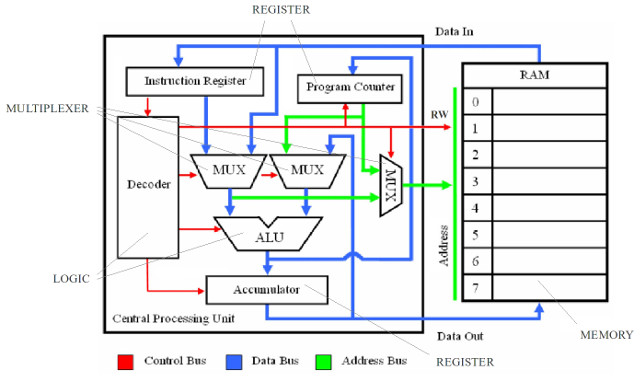
\includegraphics[scale=1]{images/cpu.jpg} 

Four fundamental components of any computer : 
\begin{itemize}
	\item Logic: every block within the computer can be considered to be made from Boolean logic gates, however, this category refers to specific larger logic blocks e.g. adders, address decoders, instruction decoders etc.
	\item Multiplexers: from one point of view a computer just moves information from one point to another. Controlling the path taken by this information are multiplexers: switching junctions, allowing information to be passed between functional blocks.
	\item Registers: fast, short term memory. As part of the Fetch-Decode-Execute cycle a computer needs to remember its state, the instruction to be processed and any results generated.
	\item Memory: this computer uses a classic Von Neumann architecture i.e. one memory, storing both the program (instructions) to be executed and the data to be processed in the same memory device.
\end{itemize}

In there simplest forms : 
\begin{itemize}
	\item A bus is just a group of wires carrying binary numbers
	\item A multiplex are switches allowing the processor to select info from multiple sources and route it to a single destination
\end{itemize}

On its own a half adder is not overly useful as we need to add 8 bit numbers, however multiple half adders can form a full adder. 

See diagram:

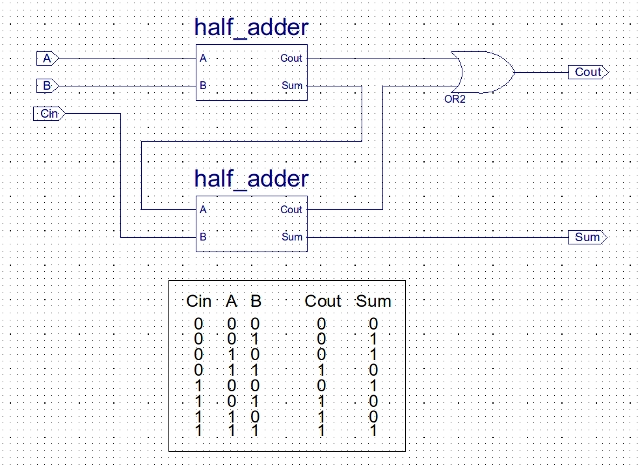
\includegraphics[scale=1]{images/half_adders.jpg}

Multiple full adders can make a ripple adder, this works as follows : 
Each full adder is a modulus 2 adder, conceptually the addition process starts with the least significant digit (LSD) and 'ripples' through the hardware to the most significant digit (MSD) i.e. bits X0 and Y0 are added together to produce a Sum Z0 and a Carry C1, this Carry is then added to the next significant digits X1 and Y1 etc.

\begin{itemize}
	\item Program Counter (PC) : 8 bit register used to store the address in memory of the current instruction being executed.
	\item Instruction Register (IR) : 16 bit register, updated at the end of the fetch phase with the instruction to be processed (decoded and executed).
	\item Accumulator (ACC) : 8 bit register, a general purpose data register, providing data (operand) to be processed by the ALU and used to store any result produced. Note, we can only store one 8 bit value at a time on the processor, other data values will need to be buffered in memory.
\end{itemize}

Jump Logic 

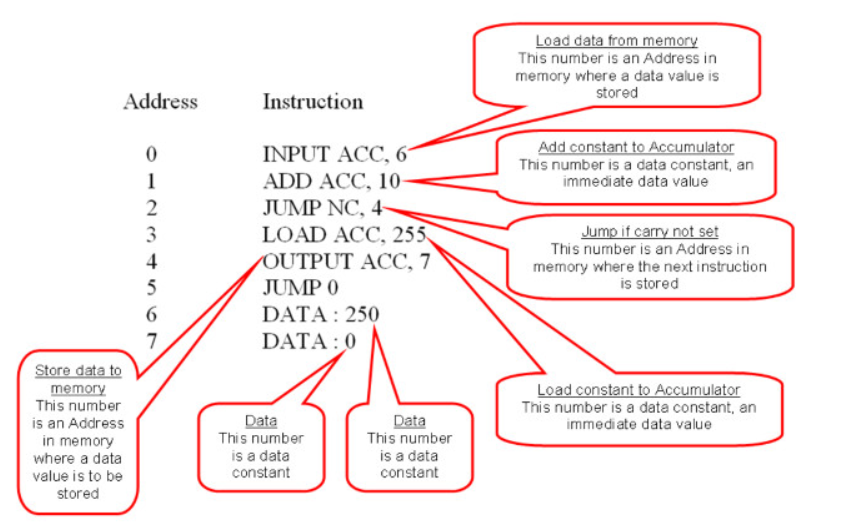
\includegraphics[scale=1]{images/jump_logic.jpg}



